\documentclass[a4paper,14pt]{extarticle}

\usepackage[default]{comfortaa}
\usepackage[utf8]{inputenc}
\usepackage[T1]{fontenc}
\usepackage[english]{babel}
\usepackage[left=0cm, right=0.5cm, bottom=0.5cm, top=0.5cm]{geometry}
\usepackage{fixltx2e}
\usepackage{graphicx}
\usepackage{amsmath}
\usepackage{amssymb}
\usepackage{mathrsfs}
\usepackage{indentfirst}
\usepackage[shortlabels]{enumitem}
\usepackage[usenames,dvipsnames]{xcolor}
\usepackage{tcolorbox}
\usepackage{marvosym}
\usepackage{genealogytree}
\usepackage{hyperref}
\usepackage{fontawesome}

%\colorlet{bgcol}{LimeGreen!40!white}
\colorlet{bgcol}{LimeGreen}
\newcommand{\circb}[1]{\begin{minipage}{1cm}
    \begin{tcolorbox}[colback=Green,colframe=Green,
        halign=flush center, valign=center, square, circular arc,
        width=0.8cm, left=0cm, right=0cm]
        {\large #1}
    \end{tcolorbox}
\end{minipage}}
\newcommand{\cvtitle}[1]{
    \begin{tcolorbox}[colback=bgcol,colframe=ForestGreen,
        height=1cm, valign=center, sharp corners=downhill]
        {\Large #1}
    \end{tcolorbox}
}
\newcommand{\gritem}{\color{bgcol}$\blacksquare$}
\renewcommand{\labelitemi}{\gritem}
\newcommand{\myspace}{{\color{LimeGreen}\dotfill}}

\renewcommand{\wp}[1]  {\begin{minipage}[b][2mm][c]{3mm} #1 \end{minipage}}
\newcommand{\skdabb} {{\color{LimeGreen}$\blacksquare$~\color{Green!20!white}$\blacksquare$~\color{OliveGreen!20!white}$\blacksquare$}}
\newcommand{\skmore} {{\color{LimeGreen}$\blacksquare$~\color{Green}$\blacksquare$~\color{OliveGreen!20!white}$\blacksquare$}}
\newcommand{\skexp}  {{\color{LimeGreen}$\blacksquare$~\color{Green}$\blacksquare$~\color{OliveGreen}$\blacksquare$}}

\begin{document}

\begin{minipage}[c]{0.35\linewidth}
    \begin{tcolorbox}[
        colback=bgcol,
        colframe=ForestGreen,
        subtitle style={
            colback=bgcol,
            coltext=black
        },
        leftrule=2mm,
        sharp corners=uphill,
        height=282mm,
    ]
        \begin{minipage}{0.45\linewidth}
            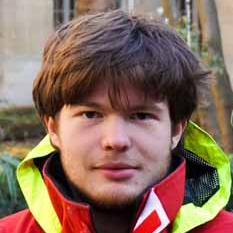
\includegraphics[width=\linewidth]{head.png}
        \end{minipage}
        \hfill
        \begin{minipage}{0.45\linewidth}
            Luc

            \textbf{Chabassier}
        \end{minipage}

        \vspace{0.2cm}
        {\small
        \circb{\gtrsymBorn}September 19, 1996 \newline
        \circb{\Telefon} +33~(0)609642210 \newline
        \circb{\Letter} \href{mailto:luc.chabassier@ens.fr}{luc.chabassier@ens.fr} \newline
        \circb{\Mundus} \href{https://dwarfmaster.net}{dwarfmaster.net} \newline
        \circb{\faGithub} \href{https://github.com/lucas8}{lucas8} \newline
        }

        \vspace{1cm}
        \tcbsubtitle{\Large\bf About me}

        A student in computer science, passionate with everything related to
        computers, who started programming for fun at the age of 14. Leaving
        the imperative paradigm he started with, he now focus mostly on
        strongly typed functional languages and formal proofs.

        \vspace{1cm}
        \tcbsubtitle{\Large\bf Interests}

        Programming, reading science fiction and fantasy, climbing and sailing.

    \end{tcolorbox}\end{minipage}
    \hfill
    \begin{minipage}[c][282mm][t]{0.60\linewidth}

        \cvtitle{Education}

        \begin{itemize}
            \item \textbf{2014} baccalauréat S with highest honours
            \item \textbf{2014-2016} Maths-Physic preparatory class at \emph{Pierre de Fermat} in Toulouse
            \item \textbf{2016+} Computer science licentiate at \emph{École Normale Supérieure} in Paris
        \end{itemize}

        \cvtitle{Experience}

        \begin{itemize}
            \item \textbf{Internship} A deriving mecanism for Coq \\
                \emph{June 2017 - August 2017} \\
                MARELLE team at INRIA Sophia-Antipolis
            \item \textbf{Project} Absint \\
                \emph{June 2017} \\
                Abstract interpreter for a subset of C
            \item \textbf{Project} Adac \\
                \emph{Semptember 2016 - January 2017} \\
                A compiler for a subset of Ada
            \item \textbf{System} NixOS package maintainer \\
                \emph{2016+}
            \item \textbf{Project} Warrior \\
                \emph{September 2013 - July 2014} \\
                Fighting game in C++
        \end{itemize}

        \cvtitle{Skills}

        \begin{itemize}
            \item \textbf{Programming languages} Haskell, C++, OCaml, \LaTeX, Assembly, Perl, Python
            \item \textbf{Tools} Bash, Git, Unix
            \item \textbf{Technologies} Coq, SQL, HTML
            \item \textbf{Knowledge} Abstract interpretation, formal proof systems, natural language semantics,
                functional programming, unix systems, convex optimisation, statistical learning
            \item \textbf{Spoken languages} native french, fluent english, basic spanish
        \end{itemize}

    \end{minipage}

\end{document}

